\documentclass[a4paper,12pt,ngerman]{scrartcl}

% Language
\usepackage{polyglossia}
\setmainlanguage{german}

% Grafiken
\usepackage{graphicx}

% Make \today print in format "NN<st|nd|rd|th> MM YYYY"
\usepackage{isodate}
\origdate

\linespread{1.15}

% Titel anders formatieren mit: Command, Format, Label, Sep, Before-Code
\usepackage{titlesec}
\titleformat{\section}{\sffamily\Large\bfseries}{}{0pt}{}
\titleformat{\subsection}{\sffamily\large\bfseries}{}{0pt}{}

% Own pagestyle (header and footer)
\usepackage{fancyhdr}
\fancyhf{} % Clear header and footer content
\fancyhead[L]{{\small \textsf{WS 14/15, Informationsvisualisierung}}}
\fancyhead[C]{{\small \textsf{Übung 1}}}
\fancyhead[R]{{\small \textsf{\today}}}
\fancyfoot[R]{{\small Jennifer Kane, Jonas Gröger}}
\fancyfoot[C]{\thepage}

% Text in quotes
% Usage: \enquote{To be or not to be.}
\usepackage{csquotes}

% Subliminal refinements towards typographical perfection
\usepackage{microtype}

% Better refs with \cref{}
\usepackage[capitalize,noabbrev]{cleveref}

% Borders
\usepackage[paper=a4paper,left=20mm,right=20mm,top=30mm,bottom=30mm]{geometry}

\begin{document}
\pagestyle{fancy} % Activate own pagestyle

\section{Aufgabe 1.1 | Design principles}

\subsection*{Data-Ink-Ratio}

Gleich zwei Diagrammarten werden in \cref{screens} kombiniert. Zwei der vier Werte werden direkt im Kreisdiagramm (Pie-Chart) dargestellt. Da der Platz für die Beschreibung der zwei kleineren Bereiche im Kreisdiagramm nicht ausreicht, wurde dort nur ein einziger Bereich ausgewiesen, der in einem zusätzlichen Balkendiagramm (Bar-Chart) weiter differenziert wird. Durch diesen unnötigen Zwischenschritt ergibt sich eine niedrige \emph{Data-Ink-Ratio}.

\begin{figure}[ht]
    \centering
    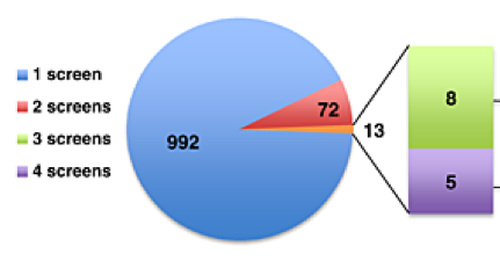
\includegraphics[width=0.6\textwidth]{includes/screens}
    \caption{Anzahl der Bildschirme}
    \label{screens}
\end{figure}

\subsection*{Lie-Factor}
\Cref{festival_sharing} stammt aus einer Reihe von Darstellungen, die das Verhalten von Festivalbesuchern im Bezug auf das Teilen von Inhalten im Internet beschreibt. In dieser speziellen Grafik geht es allein darum, von welchen Festivals aus wie viele Inhalte geteilt wurden.

\begin{figure}[ht]
    \centering
    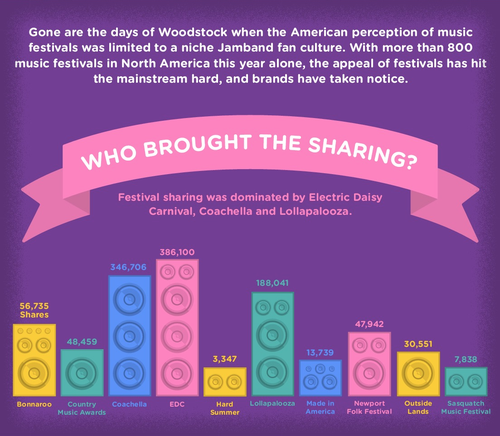
\includegraphics[width=0.73\textwidth]{includes/festival_sharing}
    \caption{Festival Sharing}
    \label{festival_sharing}
\end{figure}

Sie dient unter anderem als Beispiel für einen hohen \emph{Lie-Factor}. Beim Vergleich der Höhen der Balken ergeben sich ganz andere Verhältnisse als durch Betrachtung der  Zahlendarstellungen. Es finden sich kaum zwei Daten, deren Darstellung in angemessener Relation zu den Zahlwerten steht.
Beispiel: Vergleich von Coachella und Lollapalooza

\begin{equation}
    Lie-factor = \frac{1.2 / 1}{346\,706 / 188\,041} \approx 1.84
\end{equation}

Hinzu kommt die Gestaltung der Balken als Lautsprecherboxen, die durch die verschiedene Anzahl an Lautsprechern zusätzlich verwirrt. Auch die Farbaufteilung scheint hier Bedeutung zu verleihen, wo keine ist.

Durch die Verwendung einfacher, gleichfarbiger Balken hätte man ein eindeutiges Bild und zudem eine höhere \emph{Data-Ink-Ratio}. Auch eine Umordnung der Ergebnisse in auf- oder absteigender Reihenfolge kann die \emph{Data-Ink-Ratio} erhöhen. Dann entfällt die Notwendigkeit, zusätzlich textuell zu beschreiben, welche Festivals den größten Beitrag geleistet haben.

\subsection*{Chart-Junk}

\Cref{usa} hat nur eine einzige Aussage. Um diese künstlich aufzuplustern, wird hier die Prozentzahl der Amerikaner, die Zugang zu einer Breitbandverbindung mit mindestens 10 Mbps Download-Geschwindigkeit haben, anhand einer geographischen Abbildung der USA visualisiert. Dies ist zum einen völlig unnötig (\emph{Chart-Junk}), zum anderen wirft es eher Fragen auf, als dass es das Verständnis der Aussage erleichtert. Es sticht zunächst der graue Balken im Norden der USA ins Auge, was vermuten lässt, dass speziell dort die Abdeckung nicht gewährleistet ist. Angaben zur Bevölkerung sollen nur dann mit geographischer Lage verknüpft werden, wenn tatsächlich eine Verbindung zwischen diesen Daten besteht.

\begin{figure}[ht]
    \centering
    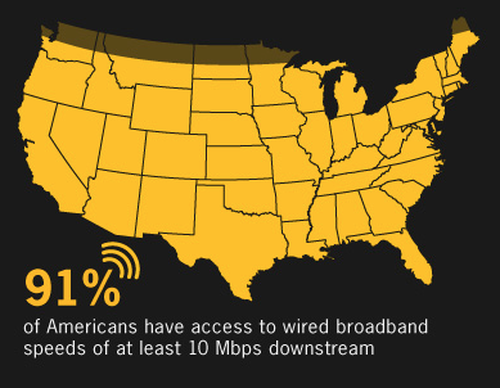
\includegraphics[width=0.5\textwidth]{includes/usa}
    \caption{Geschwindigkeit des Breitbandzugangs in den USA}
    \label{usa}
\end{figure}

Generell führt \emph{Chart-Junk} immer auch zu einer niedrigen \emph{Data-Ink-Ratio}, die auch in dieser Visualisierung sehr niedrig ist.

\section{Aufgabe 1.2 | Bewertung}

Die \Cref{water-0,water-1,water-2,water-3} zeigen Frischwasservorräte pro Land in $1.000 m^3$ pro Person. Der betrachtete Zeitraum beläuft sich dabei auf Mitte der 90er bis 2000. Alle Abbildungen sind in blau gehalten, haben einen teilweise gerasterten Hintergrund und durch Tropfen verursachte Wellen. Die Größe des Frischwasservorrats ist als Tropfen (nicht linear skaliert) repräsentiert.

\begin{figure}
    \centering
    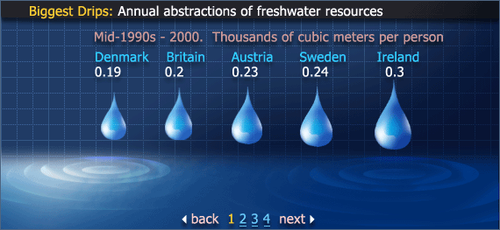
\includegraphics[width=0.7\textwidth]{includes/water-0}
    \caption{Frischwasservorrat in unterschiedlichen Ländern (1)}
    \label{water-0}
\end{figure}

\begin{figure}
    \centering
    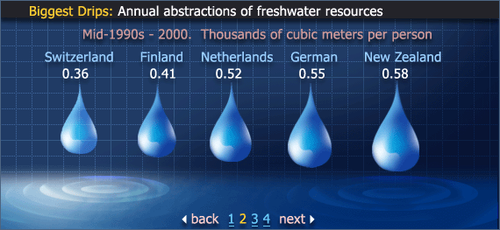
\includegraphics[width=0.7\textwidth]{includes/water-1}
    \caption{Frischwasservorrat in unterschiedlichen Ländern (2)}
    \label{water-1}
\end{figure}

\begin{figure}
    \centering
    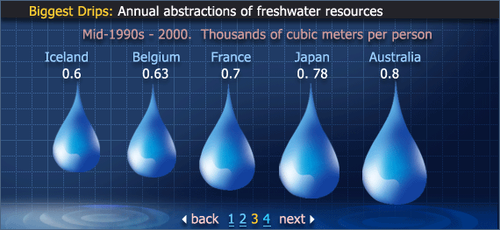
\includegraphics[width=0.7\textwidth]{includes/water-2}
    \caption{Frischwasservorrat in unterschiedlichen Ländern (3)}
    \label{water-2}
\end{figure}

\begin{figure}
    \centering
    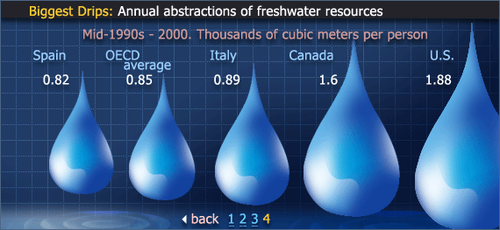
\includegraphics[width=0.7\textwidth]{includes/water-3}
    \caption{Frischwasservorrat in unterschiedlichen Ländern (4)}
    \label{water-3}
\end{figure}

Bei der Grafik wurden optische Elemente wie Tropfen mit Reflektionen und Wellen auf dem Wasser eingesetzt. Daher könnte es sein dass die Grafik für einen Artikel in einem Magazin oder einer Zeitung verwendet wurde.

Auf den ersten Blick wird in zeitlicher Reihenfolge folgendes wahrgenommen:

\begin{enumerate}
	\item Die Grafik besteht als vier Teilen, ersichtlich durch die Anzahl der Dateien noch vor betrachten der eigentlichen Grafik.
	\item Es sind Tropfen abgebildet.
	\item Der großflächige Hintergrund.
	\item Der Text über den Tropfen (z.B. Iceland 0.6)
\end{enumerate}

Probleme besitzen die Grafiken einige. Da die Länder auf vier verschiedene Grafiken verteilt sind, hat man als Betrachter keine einfache Vergleichbarkeit zwischen den Ländern. Ein schlechter Data-Ink-Ratio ist durch den großflächigen Hintergrund und die Tropfen ebenfalls gegeben. Weiterhin sind die Größen zwischen den einzelnen Ländern schwer unterscheidbar, da der Tropfen für die Zahl eine denkbar schlechte Wahl ist. Außerdem ist die Einheit (Frischwasservorräte pro Land in $1.000 m^3$ pro Person) nicht sofort erkennbar, da diese unnötig kompliziert und verteilt beschrieben wurde (\enquote{Thousands of cubic meters per person}). Eine große Anzahl von Farben und (unnötigen) Schatten wurden ebenfalls verwendet. Dazu kommt, dass Einheit und Betrachtungszeitraum in einer Zeile mit gleicher Farbe dargestellt ist. Der Zoomeffekt zwischen den vier Grafiken ist unnötig, genau so wie der Tropfen in \Cref{water-3}, der über die Zeichenfläche hinüber geht. Neben den optischen Fehlern ist noch ein logischer und ein grammatikalischer Fehler vorhanden. Die OECD, sichtbar in \Cref{water-3}, ist kein Land. Eine Hervorhebung wäre wünschenswert. Zwischen \enquote{Mid-1990s - 2000.} und \enquote{Thousands of cubic meters per person} ist bei genauer Betrachtung ein geringerer Abstand als bei den anderen drei Grafiken.

Eine alternative Darstellung wäre ein gewöhnliches Bar-Chart wie in \Cref{frischwasser-bar} dargestellt.

\begin{figure}
    \centering
    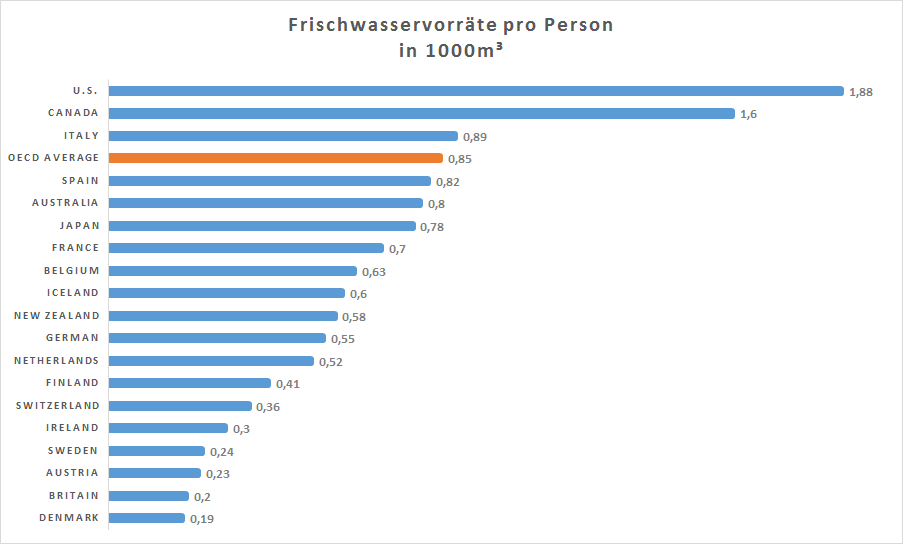
\includegraphics[width=0.9\textwidth]{includes/frischwasser-bar}
    \caption{Bar-Chart zur Darstellung der Frischwasservorräte pro Land in $1.000 m^3$ pro Person}
    \label{frischwasser-bar}
\end{figure}

\end{document}
